\documentclass[journal,12pt,twocolumn]{IEEEtran}

\usepackage{setspace}
\usepackage{gensymb}
\singlespacing
\usepackage[cmex10]{amsmath}

\usepackage{amsthm}

\usepackage{mathrsfs}
\usepackage{txfonts}
\usepackage{stfloats}
\usepackage{bm}
\usepackage{cite}
\usepackage{cases}
\usepackage{subfig}

\usepackage{longtable}
\usepackage{multirow}

\usepackage{enumitem}
\usepackage{mathtools}
\usepackage{steinmetz}
\usepackage{tikz}
\usepackage{circuitikz}
\usepackage{verbatim}
\usepackage{tfrupee}
\usepackage[breaklinks=true]{hyperref}
\usepackage{graphicx}
\usepackage{tkz-euclide}

\usetikzlibrary{calc,math}
\usepackage{listings}
    \usepackage{color}                                            %%
    \usepackage{array}                                            %%
    \usepackage{longtable}                                        %%
    \usepackage{calc}                                             %%
    \usepackage{multirow}                                         %%
    \usepackage{hhline}                                           %%
    \usepackage{ifthen}                                           %%
    \usepackage{lscape}     
\usepackage{multicol}
\usepackage{chngcntr}

\DeclareMathOperator*{\Res}{Res}

\renewcommand\thesection{\arabic{section}}
\renewcommand\thesubsection{\thesection.\arabic{subsection}}
\renewcommand\thesubsubsection{\thesubsection.\arabic{subsubsection}}

\renewcommand\thesectiondis{\arabic{section}}
\renewcommand\thesubsectiondis{\thesectiondis.\arabic{subsection}}
\renewcommand\thesubsubsectiondis{\thesubsectiondis.\arabic{subsubsection}}


\hyphenation{op-tical net-works semi-conduc-tor}
\def\inputGnumericTable{}                                 %%

\lstset{
%language=C,
frame=single, 
breaklines=true,
columns=fullflexible
}
\begin{document}


\newtheorem{theorem}{Theorem}[section]
\newtheorem{problem}{Problem}
\newtheorem{proposition}{Proposition}[section]
\newtheorem{lemma}{Lemma}[section]
\newtheorem{corollary}[theorem]{Corollary}
\newtheorem{example}{Example}[section]
\newtheorem{definition}[problem]{Definition}

\newcommand{\BEQA}{\begin{eqnarray}}
\newcommand{\EEQA}{\end{eqnarray}}
\newcommand{\define}{\stackrel{\triangle}{=}}
\bibliographystyle{IEEEtran}
\raggedbottom
\setlength{\parindent}{0pt}
\providecommand{\mbf}{\mathbf}
\providecommand{\pr}[1]{\ensuremath{\Pr\left(#1\right)}}
\providecommand{\qfunc}[1]{\ensuremath{Q\left(#1\right)}}
\providecommand{\sbrak}[1]{\ensuremath{{}\left[#1\right]}}
\providecommand{\lsbrak}[1]{\ensuremath{{}\left[#1\right.}}
\providecommand{\rsbrak}[1]{\ensuremath{{}\left.#1\right]}}
\providecommand{\brak}[1]{\ensuremath{\left(#1\right)}}
\providecommand{\lbrak}[1]{\ensuremath{\left(#1\right.}}
\providecommand{\rbrak}[1]{\ensuremath{\left.#1\right)}}
\providecommand{\cbrak}[1]{\ensuremath{\left\{#1\right\}}}
\providecommand{\lcbrak}[1]{\ensuremath{\left\{#1\right.}}
\providecommand{\rcbrak}[1]{\ensuremath{\left.#1\right\}}}
\theoremstyle{remark}
\newtheorem{rem}{Remark}
\newcommand{\sgn}{\mathop{\mathrm{sgn}}}
\providecommand{\abs}[1]{\left\vert#1\right\vert}
\providecommand{\res}[1]{\Res\displaylimits_{#1}} 
\providecommand{\norm}[1]{\left\lVert#1\right\rVert}
%\providecommand{\norm}[1]{\lVert#1\rVert}
\providecommand{\mtx}[1]{\mathbf{#1}}
\providecommand{\mean}[1]{E\left[ #1 \right]}
\providecommand{\fourier}{\overset{\mathcal{F}}{ \rightleftharpoons}}
%\providecommand{\hilbert}{\overset{\mathcal{H}}{ \rightleftharpoons}}
\providecommand{\system}{\overset{\mathcal{H}}{ \longleftrightarrow}}
	%\newcommand{\solution}[2]{\textbf{Solution:}{#1}}
\newcommand{\solution}{\noindent \textbf{Solution: }}
\newcommand{\cosec}{\,\text{cosec}\,}
\providecommand{\dec}[2]{\ensuremath{\overset{#1}{\underset{#2}{\gtrless}}}}
\newcommand{\myvec}[1]{\ensuremath{\begin{pmatrix}#1\end{pmatrix}}}
\newcommand{\mydet}[1]{\ensuremath{\begin{vmatrix}#1\end{vmatrix}}}
\numberwithin{equation}{subsection}

\makeatletter
\@addtoreset{figure}{problem}
\makeatother
\let\StandardTheFigure\thefigure
\let\vec\mathbf

\renewcommand{\thefigure}{\theproblem}

\def\putbox#1#2#3{\makebox[0in][l]{\makebox[#1][l]{}\raisebox{\baselineskip}[0in][0in]{\raisebox{#2}[0in][0in]{#3}}}}
     \def\rightbox#1{\makebox[0in][r]{#1}}
     \def\centbox#1{\makebox[0in]{#1}}
     \def\topbox#1{\raisebox{-\baselineskip}[0in][0in]{#1}}
     \def\midbox#1{\raisebox{-0.5\baselineskip}[0in][0in]{#1}}
\vspace{3cm}
\title{Assignment-1C}
\author{ BANDI SAI LAXMAN - EE18BTECH11049}
\maketitle
\newpage
\renewcommand{\thefigure}{\theenumi}
\renewcommand{\thetable}{\theenumi}


%%%%%%

\section{Software Installation}
Run the following commands
\begin{lstlisting}
sudo apt-get update
sudo apt-get install libffi-dev libsndfile1 python3-scipy  python3-numpy python3-matplotlib 
sudo pip install cffi pysoundfile 
\end{lstlisting}

Make sure gcc is Installed ,  compile and execute using below commands 
\begin{lstlisting}
gcc file.c -o file -lm
./file
\end{lstlisting}



\section{Digital Filter}
\begin{enumerate}[label=\thesection.\arabic*
,ref=\thesection.\theenumi]
\item
\label{prob:input}
Download the sound file from  
\begin{lstlisting}
wget https://raw.githubusercontent.com/gadepall/ 
EE1310/master/filter/codes/Sound_Noise.wav
\end{lstlisting}

\item
\label{prob:input}
Generate .dat file From the above sound file 
\begin{lstlisting}
codes/generate_dat.py

\end{lstlisting}


\item
\label{prob:output}
Write the python code for removal of out of band noise and execute the code.
\\
\solution
\lstinputlisting{./codes/butter_remove.py}
%%%%%%%


\end{enumerate}








\section{Difference equation}

\begin{enumerate}[label=\thesection.\arabic*,ref=\thesection.\theenumi]
\item
\label{prob:diffEq}
Write the difference equation of the above Digital filter obtained in problem \ref{prob:output}.
\\
\solution
\begin{equation}
\label{eq:eqn1}
 \sum _{m=0}^{M}a\brak{m}y\brak{n-m}=\sum _{k=0}^{N}b\brak{k}x\brak{n-k}
\end{equation}
\begin{equation}
\label{eq:eqn2}
\begin{split}
y(n) - 2.52y(n-1) + 2.56y(n-2) - 1.206y(n-3)
\\
+ 0.22013y(n-4) = 0.00345x(n) + 0.0138x(n-1)
\\
+ 0.020725x(n-2) + 0.0138x(n-3) + 0.00345x(n-4)
\end{split}
\end{equation}



\end{enumerate}
%%%%%%
\section{Z-transform}

\begin{enumerate}[label=\thesection.\arabic*,ref=\thesection.\theenumi]


\item 
\label{prob:fft_c}
Find fourier Transform of $x(n)$ and $h(n)$ obtained using difference equation in problem \ref{prob:diffEq} using C . 

\solution 

$x(n)$ =  audio signal input  \\
$h(n)$ = filter.\\

Convolution : $y(n) = x(n)*h(n)$, 
\\
Taking Fourier Transform, we get:
\\
$Y(K) = H(K) X(K)$ \\
\\
$x(n)$ will be generated from Sound\_Noise.wav. 


$h(n)$ is generated using the equation in problem  \ref{prob:diffEq}  .





To obtain the Fourier transform in $O(nlogn)$ , we break the $N$ point DFT into 2 - $N/2$ point DFT recursively.

The code to find the Fourier Transform of $x(n)$ and $h(n)$ can be found here. Generates dat files for X , H  . 
\begin{lstlisting}
codes/fft_x_h.c
\end{lstlisting}

generating FFT plots of x(n) and h(n) 


\begin{figure}[!ht]
\centering
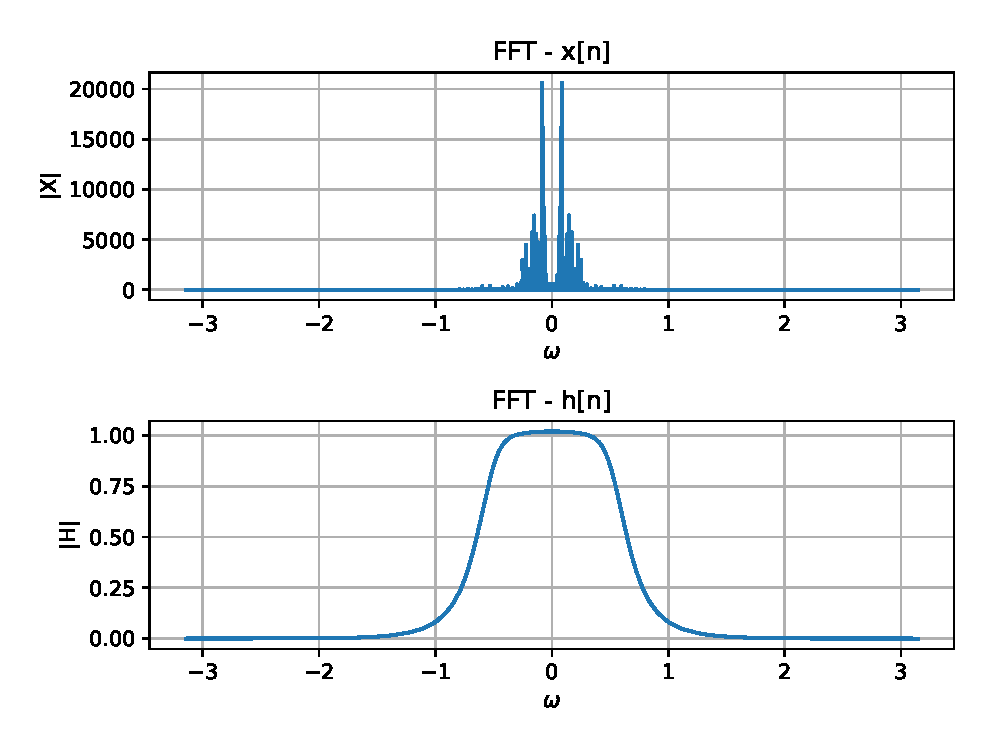
\includegraphics[width=\columnwidth]{figs/fft_h}
\caption{FFT of x(n) and h(n)}
\label{fig:2}
\end{figure}

\textbf{Verification}:

 we obtain the Inverse Fourier Transform of Y(K) to obtain y(n) and the filtered sound. 

\begin{lstlisting}
codes/ifft_Y.c
\end{lstlisting}


\begin{figure}[!ht]
\centering
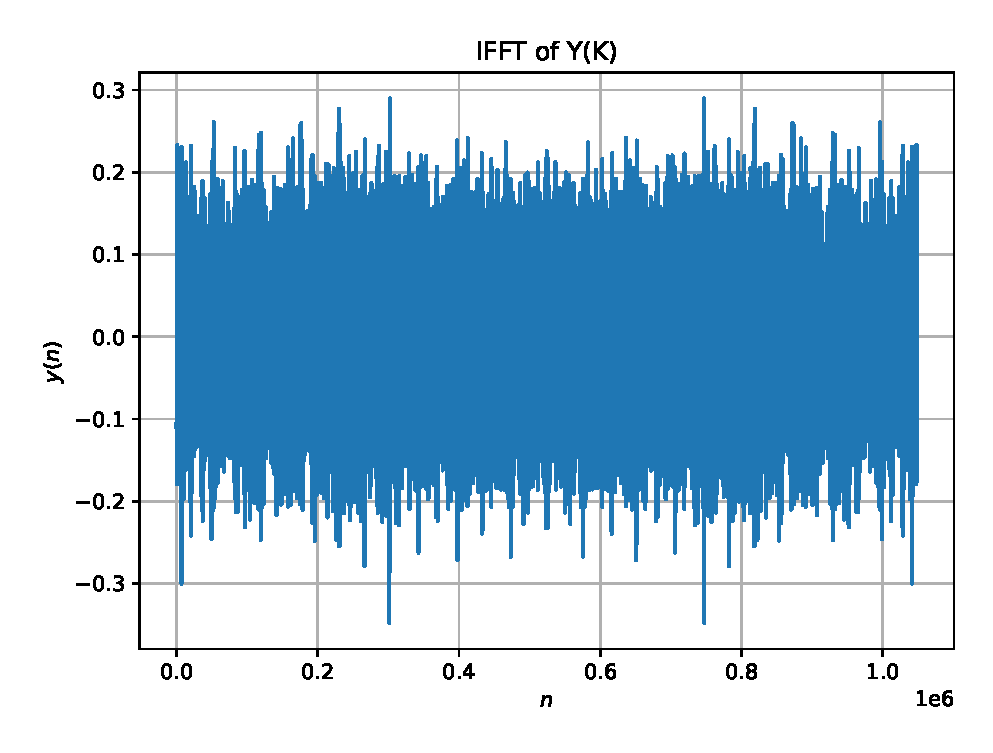
\includegraphics[width=\columnwidth]{figs/ifft_y}
\caption{IFFT - Y(K)}
\label{fig:2}
\end{figure}


It looks similar to the plots generated from the in built function of IFFT.\\



The code to obtain these plots.
\begin{lstlisting}
codes/plotX_H.py
codes/plot_y.py
\end{lstlisting}



\end{enumerate}


\end{document}

